\section{Contrôle des moteurs}
\begin{frame}
  \frametitle{Présentation des moteurs}
  \begin{columns}[T]
    \begin{column}{.65\textwidth}
           \begin{itemize}
            \item Moteurs utilisés 
            \begin{itemize}
              \item AX-12~ ( 12 kg.cm\up{-1})
              \item MX-28 ( 28 kg.cm\up{-1})
            \end{itemize}
            \item Avantages:
            \begin{itemize}
              \item Bus TTL , une sortie pour tous les moteurs
              \item Communication par bus UART
              \item Gestion de moteur indépendamment ou global
            \end{itemize}
          \item Inconvénient:
            \begin{itemize}
              \item Les AX-12 n'ont pas assez de couple
              \item Contrôle PID intégré réglé sans charge
              \item Moteur pas à pas
            \end{itemize}
          \end{itemize}
        \end{column}
        \begin{column}{.3\textwidth}
          \begin{figure}[ht]
            \centering
            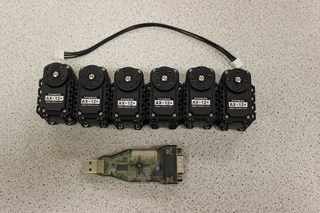
\includegraphics[scale= 0.35]{../img/AX12+USB_2_DynamicCell.JPG}
          \end{figure}
        \end{column}
      \end{columns}

\end{frame}

\begin{frame}
  \frametitle{Génération de trajectoire}
            \begin{figure}
                \begin{center}
                    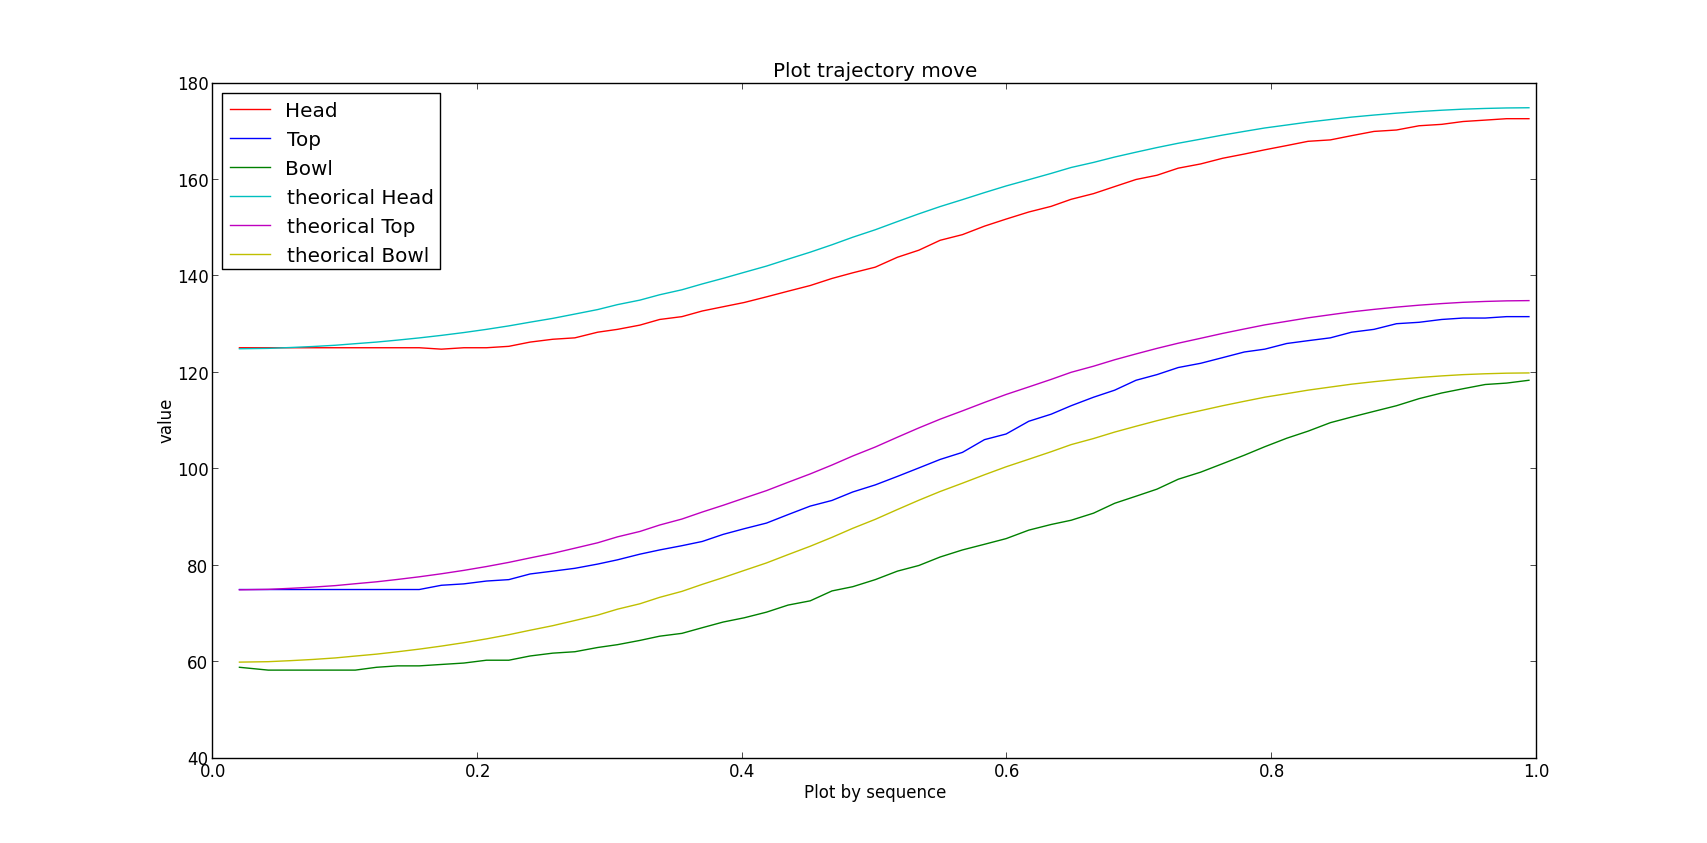
\includegraphics[width=11cm]{../img/TrajectoryPlot.png}
                \end{center}
                \caption{Exemple de résultat}
            \end{figure}
\end{frame}
